\documentclass{article}
\usepackage{graphicx}
\usepackage{hyperref} 

\usepackage[utf8]{inputenc}
\usepackage{csquotes}
\usepackage[
  backend=biber,
  style=authoryear,
  maxcitenames=1,
  natbib=true,        
  doi=false,           
  isbn=false           
]{biblatex}

\usepackage[title]{appendix}
\usepackage{float}
\usepackage{xcolor}

\usepackage{subcaption}

\usepackage[english]{babel}

\addbibresource{references.bib}
\usepackage{cleveref} 

\title{Answering Reading Comprehension Questions – Eye Tracking Based Behavior Analysis}
\date{}
\author{By Diana Morgan, Supervised by Yevgeni Berzak}

%%% change template
%%% eye movement papers from previous years (in CHI) 


%%% intro: reading, reading understending exams
%%% related work: requires effort. Non ordinary reading eye movements. Strategies references (doesn't have to be eyes). + the papers I have on dwell times.  
%%% not methods - experimental setup or something. Look at other onestop papers. # ppl, answers, texts - stats! Questions - length, num words etc. If critical spans - also adress.
%%% ABCD is very important, num answers stats, screen locations. 
%%% Data segment - 3.1
%%% After we see some difference (dwell times, simpler bit) and only then do the sequence building - now get from means to temporal part. Define agregations. Build a visualisation for sequence making w1 w2 w3 -> A/1 A/1 B/2 -> A/1 B/2

%% Simplified -> Collapsed

%%% Lots of figure work

%%% Put all Gatherers in apendix. Write - fig blah shows hunters, gatheres in apendix

%%% all the pics - to pdf


\begin{document}
\maketitle


\section{Abstract}
This paper investigates eye‐movement behavior during multiple‐choice reading comprehension tasks using the OneStop Eye Movements dataset. We analyze the fixation sequences and dwell times of 360 native English participants as they select among four answer options presented in a diamond layout. Results show that readers overwhelmingly adopt a clockwise first‐scan heuristic, beginning with the top option and proceeding around the display, independent of whether they preview the question before reading (Hunting) or after (Gathering). Individual participants typically repeat one dominant scan strategy across trials, indicating stable within‐subject heuristics. Final fixations strongly align with the selected answer (approximately 70\% of trials), and mean dwell time is consistently higher on the chosen option than on distractors. These findings highlight the role of simple spatial heuristics and gaze bias in multiple‐choice decision making and suggest that eye‐tracking provides reliable markers of emerging preferences in comprehension assessment contexts.

\section{Introduction}
    Eye‐tracking has become a powerful tool for uncovering the underlying processes of decision making, including the tasks where individuals make decisions from multiple options presented. By documenting where and when people look, researchers can infer which pieces of information attract attention, how evidence is accumulated over time, and ultimately how choices are made.

    In reading specifically, most eye‐tracking research has concentrated on how readers allocate attention to continuous text. Such studies typically track regressions, skip rates, and fixation durations as participants move through paragraphs or passages. By contrast, far fewer inquiries have been made into what happens once readers finish a text and are presented with post‐reading questions. In standardized testing or comprehension experiments, the moment when a reader encounters a multiple‐choice question represents a qualitatively different task: instead of parsing new textual information, they must compare discrete answer options and decide which best matches their understanding of the passage. By emphasizing the post‐reading question phase, our study fills this gap, revealing how examinees shift from reading‐based processing to choice‐based scanning. 
    
    In the present study, we analyze eye‐tracking data from the OneStop Eye Movements dataset published by \cite{berzak2025onestop}, which contains 360 native English speaking participants answering multiple‐choice reading‐comprehension questions. After excluding repeated readings, we analyze page 4 of each trial—where four answer options appear in a diamond shape and participants select them via a gamepad.

    We address three core questions. First, do participants follow a systematic scan path—such as a location-based clockwise sweep—when initially exploring the four answer regions? Second, once a particular scan order emerges, does each reader reliably repeat it across multiple items? Third, regardless of whether the question appears before (“Hunting”) or after (“Gathering”) reading the passage, do the final fixation and total dwell time consistently favor the chosen answer?

    Our results reveal a robust clockwise scan heuristic: the most common first-scan order is top $\to$ right $\to$ bottom $\to$ left, regardless of whether participants preview the question. Individual participants tend to repeat their chosen scan order on a majority of trials. Moreover, the final fixation aligns closely with the chosen answer (68\% of Hunting trials; 71\% of Gathering trials), and mean dwell time is significantly higher on the selected region, irrespective of reading regime. Collectively, these findings demonstrate that (a) scanning order reflects a simple spatial rule rather than correctness information, (b) each examinee typically adheres to a stable heuristic throughout the session, and (c) gaze bias toward the chosen answer emerges even when participants have no foreknowledge of the question.

    By integrating both sequence‐based and dwell‐time analyses, our study advances theoretical knowledge and offers practical insights. Theoretically, identifying a consistent clockwise scanning pattern addresses a gap in how readers explore four‐option displays. Practically, demonstrating that final fixations and dwell‐time biases reliably forecast the chosen answer. In sum, our findings highlight the power of eye‐tracking to uncover subtle decision‐making strategies and provide a replicable framework for examining scan order and gaze bias in multi‐choice scenarios.

\section{Methods}
    \subsection{OneStop Dataset}
    This research utilizes the OneStop Eye Movements dataset  \parencite{berzak2025onestop}, a large-scale corpus of eye-tracking data collected from participants reading English texts and answering corresponding reading comprehension questions.

    The data collection experiment incorporates a number of experimental manipulations, of which one is incorporated into our exploration:

    Reading Regime:
    \begin{itemize}
        \item Hunting: Participants view the question before reading the paragraph.
        \item Gathering: Participants read the paragraph before seeing the question.
    \end{itemize}

    Further, the trials of repeated readings were excluded from this analysis.
    \newline
    
    The experimental design involves participants navigating through a sequence of screens with no option to return to the previous page:
    \begin{itemize}
        \item Page 1 (Hunting regime only): A "question preview" is displayed.
        \item Page 2: A text paragraph is presented (Gathering participants start here).
        \item Page 3: A comprehension question is displayed.
        \item Page 4: Four possible answer choices are presented (in addition to the question that remains on the screen).
    \end{itemize}

    Here, we focus on page 4, which displays the four multiple-choice options.
    
    Throughout the run of the experiment, the participants control the transition between pages, as well as select their answers, using a Logitech Gamepad F310 controller with a standard diamond shaped four-button layout of the directional pad. The questions are displayed on the screen in the correspondent diamond arrangement.  

    The multiple choice answer options follow a consistent answer structure described in STRAC annotation guidelines \parencite{berzak2020starc}, where:\\
    \textbf{A} is a correct answer, based on the critical span of the text.\\
    \textbf{B} is a distractor, representing a plausible miscomprehension of the correct critical span. \\
    \textbf{C} is a distractor, based on an additional span in the text, different from the critical span. \\
    \textbf{D} is a distractor, with no support in the text.
    
    
    \subsection{Sequence Construction}
    The dataset includes individual fixations data upon words denoted Interest Areas (IA). Each word can be either a part of the Question text or part of one of the Multiple Choice Options presented. This information was aggregated, to create Trial Fixation Sequences in two major modes:
    \begin{itemize}
        \item Area Label Sequence: sequence with five possible values: "question", "answer\_A", "answer\_B", "answer\_C", and "answer\_D", where letters of the answer correspond to its "correctness" as defined by the STRAC annotations. 
        \item Screen Location Sequence: sequence with five possible values: "question", "answer\_0", "answer\_1", "answer\_2", and "answer\_3", where numbers denote the location of the answer on the screen when it was presented to the participant. Answer 0 is the top of the diamond, answer 1 is in the second row to the left, answer 2 is in the second row to the right, and answer 3 is located at the bottom of the diamond. These locations correspond to the original dataset definitions. 
    
    \end{itemize}
    Although both sequences encode the same underlying fixations, they offer two perspectives: one based on answer correctness (Label Sequence) and one based on spatial arrangement (Location Sequence). 
    
    Because nearly all trials began with one fixation on the question (left over from page 3), we discard that initial fixation so that our sequences reflect genuine scanning on page 4.

    See Appendix~\ref{app:fixseq} for a visualization of fixation sequences for a random participant. 

    
    \subsection{Sequence Manipulations}

    To allow for comparison between sequences over different text-question pairs a further simplification was performed. Simplified Fixation Sequences collapse the consecutive fixations in the same segment (consecutive identical labels) into a singular value. The resulting shorter sequence represents the "order of visitations" in areas, unaffected by the texts length. This simplification was performed for both Label and Location based sequences. By collapsing consecutive fixations in the same region, we focus on the order of visits rather than fixation duration, making sequences comparable across trials of varying length.


\section{Results}
    \subsection{First-scan Sequence Strategies}
    We start by analyzing the First-Scan Sequence -- the order in which the five segments (question and four answers) were visited by the participants. We wish to test if there exists a strategic approach to the Answer-Scanning behavior that could shed light on the cognitive processing behind the task presented to the participants. 

    Figure~\ref{fig:hunt_first_loc} showcases the result of this examination from the location perspective in Hunting regime subjects. From each trial the order of area visits was extracted, these (up to) five long sequences were enumerated, and frequency of appearance for each Screen Location at each ordered position was counted. In every answer-selected subgroup, and in both Hunting and Gathering regimes, we see the same most-commonly encountered order position (only Hunting subjects are shown; Gatherers exhibit the same pattern): answer 0 is most commonly visited first, answer 2 is most commonly visited second, then answer 3, followed by answer 1 (questions are most commonly visited last, and often not viseted at all). This sequence corresponds to a clock-wise scan from the top, in the diamond shaped displayed answers.

    To strengthen our conclusion we perform a Lag-sequential analysis, testing wether certain from $\to$ to fixations occur more often than chance \parencite{bakeman1995log}.

    Screen-location codes (answer\_0 -- answer\_3): The lag-1 Z-matrix revealed extremely large positive Z-scores (e.g. Z  $\approx$ 437 for answer\_0 $\to$ answer\_2, Z $\approx$ 550 for answer\_2 $\to$ answer\_3, Z  $\approx$ 393 for answer\_3 $\to$ answer\_1), confirming a highly significant “clockwise” scan order (top to right to bottom to left). See Appendix~\ref{app:lsa_location} for the full Z-scores table.

    \begin{figure}[H]
          \centering
          \begin{subcaptionbox}{Screen Location - A \label{fig:a}}[0.45\textwidth]
            {\centering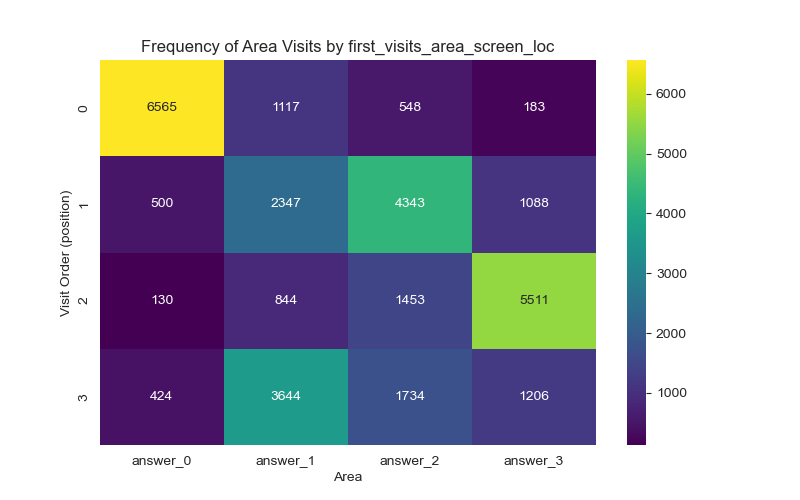
\includegraphics[width=\linewidth]{plots/visits/matrix__first_visits_area_screen_loc_hunters_A.png}}
          \end{subcaptionbox}
          \hfill
          \begin{subcaptionbox}{Screen Location - B\label{fig:b}}[0.45\textwidth]
            {\centering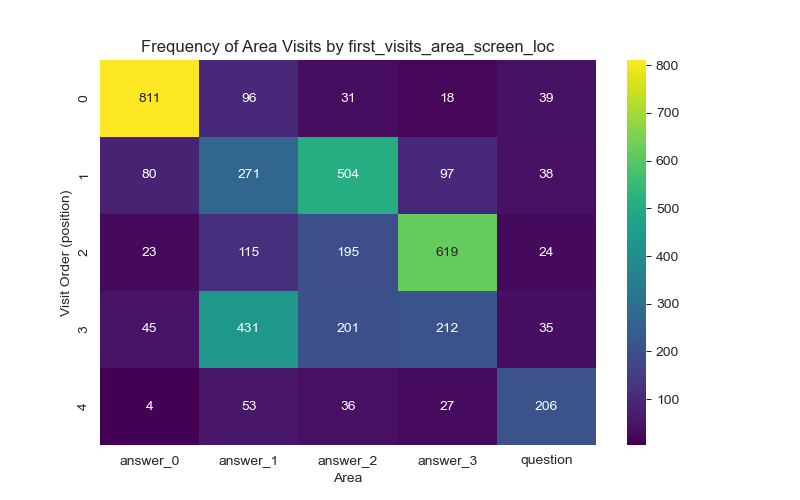
\includegraphics[width=\linewidth]{plots/visits/matrix__first_visits_area_screen_loc_hunters_B.png}}
          \end{subcaptionbox}
          
          \vspace{1em} 
        
          \begin{subcaptionbox}{Screen Location - C\label{fig:c}}[0.45\textwidth]
            {\centering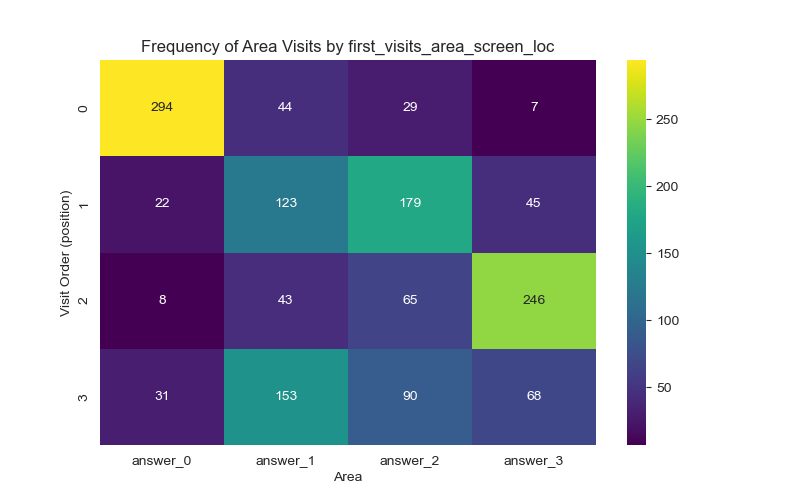
\includegraphics[width=\linewidth]{plots/visits/matrix__first_visits_area_screen_loc_hunters_C.png}}
          \end{subcaptionbox}
          \hfill
          \begin{subcaptionbox}{Screen Location - D\label{fig:d}}[0.45\textwidth]
            {\centering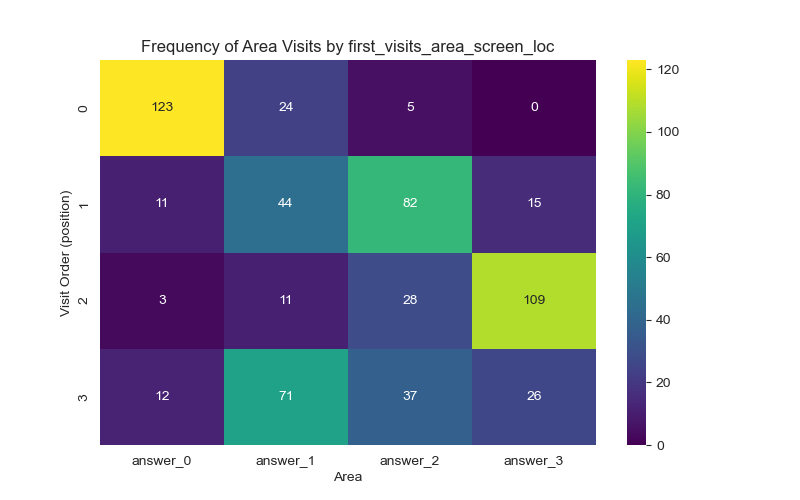
\includegraphics[width=\linewidth]{plots/visits/matrix__first_visits_area_screen_loc_hunters_D.png}}
          \end{subcaptionbox}
          
          \caption{First Five Segments Visited by Hunting Regime Participants. Each cell is a number of occurrences of given Screen Location in one of the five top positions.}
          \label{fig:hunt_first_loc}
        \end{figure}

% is clockwise correlated with how fast they find the answer? do those who are better read less? more? 

        Next, we repeat the same analysis from the correctness (Area Label) point of view. As seen in Figure~\ref{fig:hunt_first_lbl} no clear pattern emerges. It corresponds with our intuition, as the participant would have no knowledge of the "correctness" of the answers on their first scan.

        We again perform the lag-sequential analysis with lag-1. The corresponding Z-scores were all of moderate magnitude (+80 to +204) with no single positive cell dominating. This quantitatively confirms that, when viewed by correctness, there is no single “A $\to$ B” or “B $\to$ C” pattern much larger than the others.  See Appendix~\ref{app:lsa_label} for the full Z-scores table.
        
        \begin{figure}[H]
          \centering
          \begin{subcaptionbox}{Area Label - A \label{fig:aa}}[0.45\textwidth]
            {\centering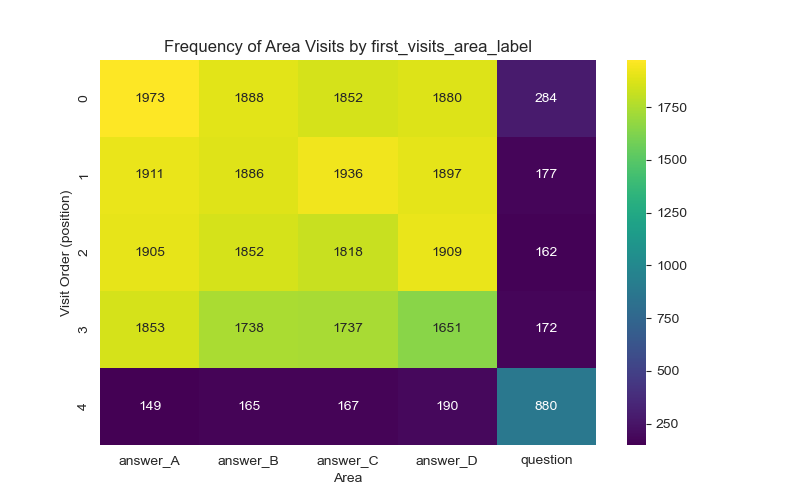
\includegraphics[width=\linewidth]{plots/visits/matrix__first_visits_area_label_hunters_A.png}}
          \end{subcaptionbox}
          \hfill
          \begin{subcaptionbox}{Area Label - B\label{fig:bb}}[0.45\textwidth]
            {\centering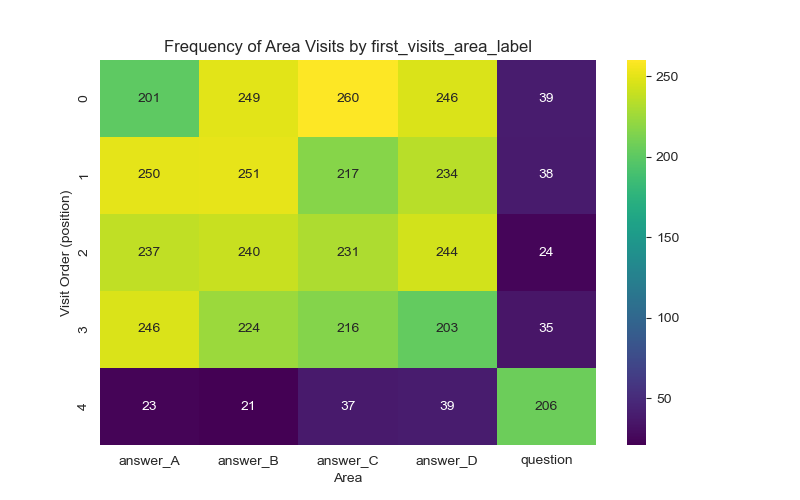
\includegraphics[width=\linewidth]{plots/visits/matrix__first_visits_area_label_hunters_B.png}}
          \end{subcaptionbox}
          
          \vspace{1em}
        
          \begin{subcaptionbox}{Area Label - C\label{fig:cc}}[0.45\textwidth]
            {\centering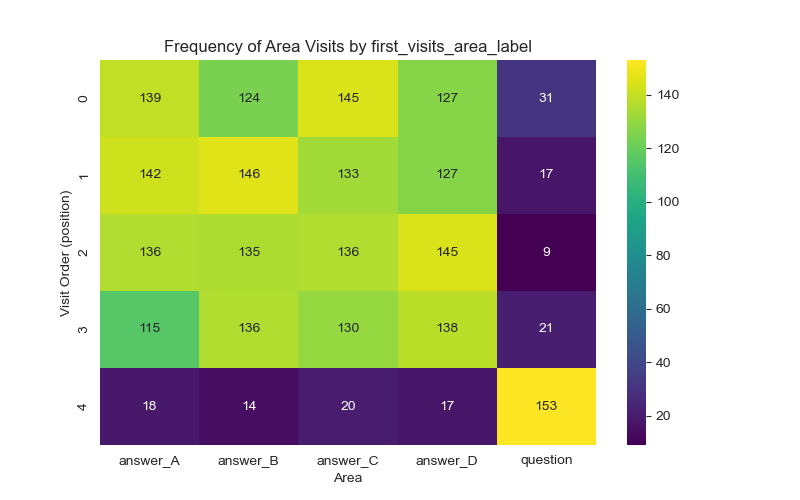
\includegraphics[width=\linewidth]{plots/visits/matrix__first_visits_area_label_hunters_C.png}}
          \end{subcaptionbox}
          \hfill
          \begin{subcaptionbox}{Area Label - D\label{fig:dd}}[0.45\textwidth]
            {\centering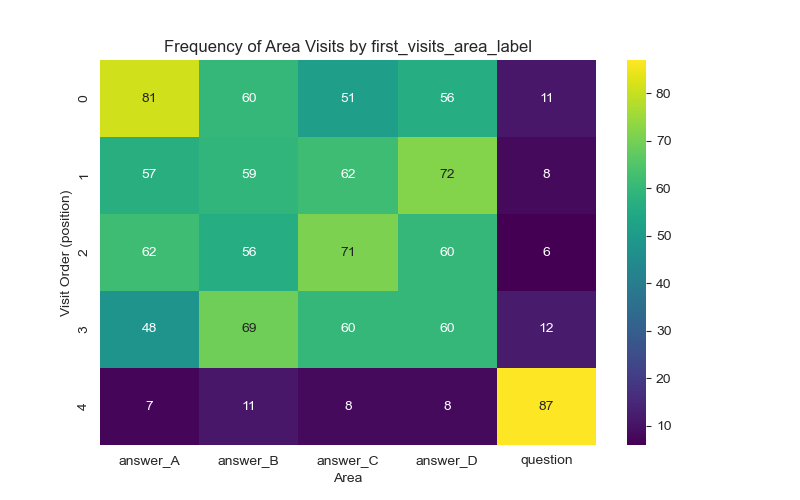
\includegraphics[width=\linewidth]{plots/visits/matrix__first_visits_area_label_hunters_D.png}}
          \end{subcaptionbox}
          
          \caption{First Five Segments Visited by Hunting Regime Participants. Each cell is a number of occurrences of given Area Label in one of the five top positions.}
          \label{fig:hunt_first_lbl}
        \end{figure}


        We continue by removing the "question" value out of the sequences, to simplify the exploration to the answers-scanning only, and we look at most dominant strategies present in the data.

        Figure~\ref{fig:A_hunt_frst_loc} shows the 35 most common first-scan strategies (by screen location). We can see that the frequency of use diminishes rapidly, with top-3 most common strategies being (1) clock-wise from the top, (2) counter-clockwise from the top, (3) zigzag (numbering of questions order), with clockwise being the clearly most common strategy. These top three strategies remain consistent across all answer-selected subgroups for both Hunters and Gatherers, with only deviation being Hunters who answered D where zigzag strategy is instead the fourth most common, overtaken by clock-wise from the left (fourth most common). 

        \begin{figure}[H]
            \centering
            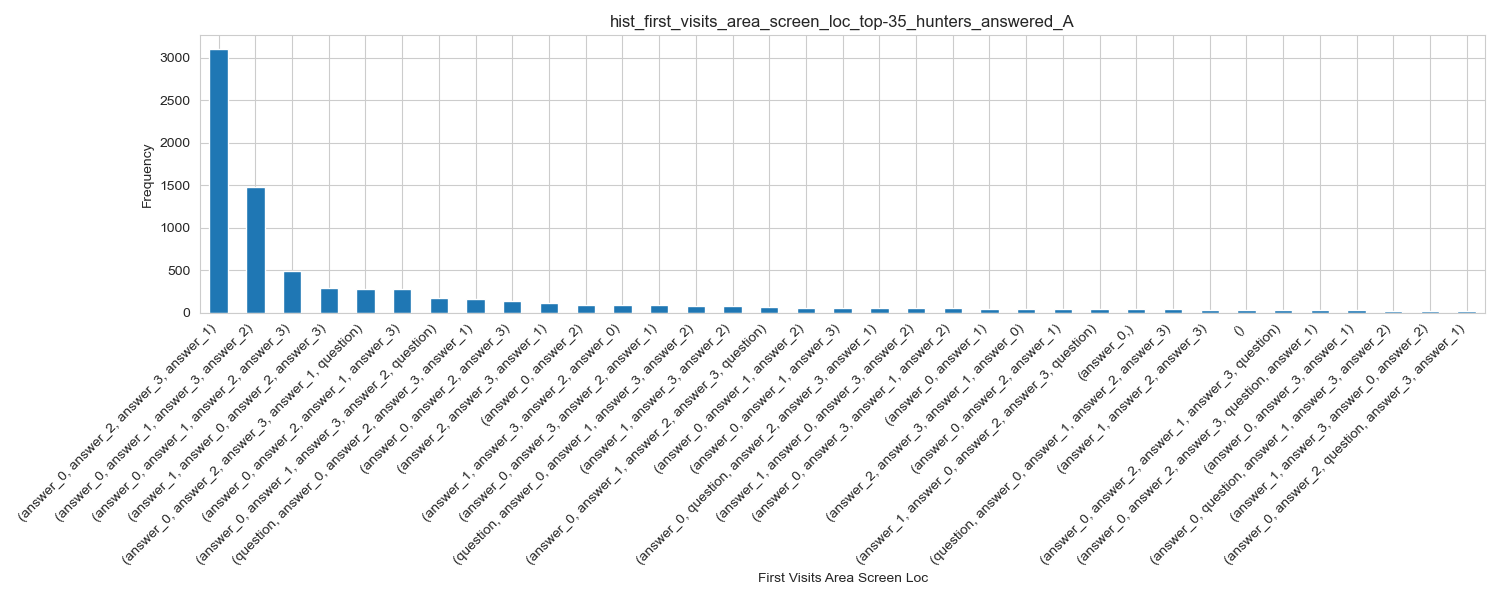
\includegraphics[width=1\linewidth]{plots/visits_hists/hist_first_visits_area_screen_loc_top-35_hunters_answered_A.png}
            \caption{First Visits by Screen Location (Hunting participants who answered A)}
            \label{fig:A_hunt_frst_loc}
        \end{figure}

        We see an approximately even distribution across all 4-long scan strategies by Area Label (Figure~\ref{fig:A_hunt_frst_lbl})

        \begin{figure}[H]
            \centering
            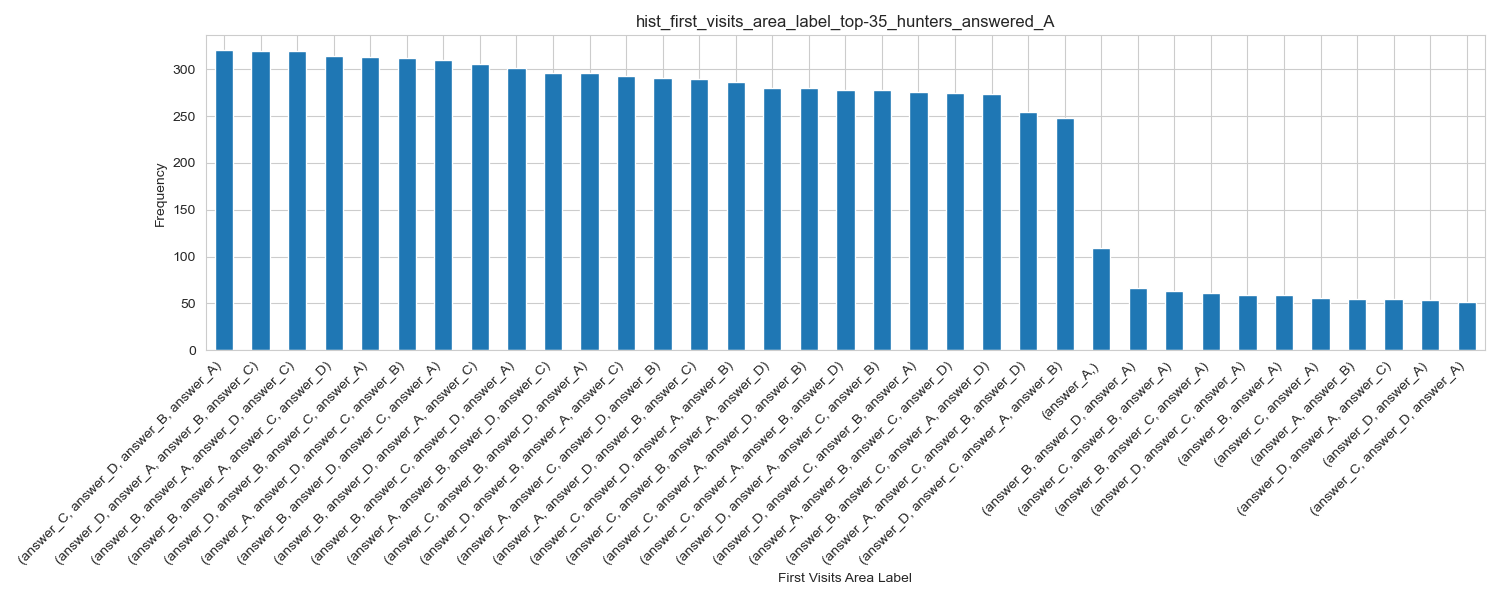
\includegraphics[width=1\linewidth]{plots/visits_hists/hist_first_visits_area_label_top-35_hunters_answered_A.png}
            \caption{First Visits by Area Label (Hunting participants who answered A)}
            \label{fig:A_hunt_frst_lbl}
        \end{figure}
        
    \subsection{Consistency in Strategy Selection}   
    We aim to further explore the common First-Scan strategies by asking if the behavior remains consistent across trials for a given participant. For each participant, we identify their Dominant First-Scan Strategy as the four-element sequence they used most often across trials. In Figure~\ref{fig:dom_props} you can see the proportion of trials the Dominant Strategy was used in. We note that Gathering regime participants show greater consistency in use of their dominant strategy (use their dominant strategy in greater proportion of trials).} 

    Furthermore, we examine which strategies are most often dominant. Among both Hunting and Gathering participants who used their Dominant Strategy in at least half of the trials, the same top three strategies emerge to be most common ones as in the general population.


     \begin{figure}[H]
          \centering
          \begin{subcaptionbox}{Proportion of trials most common strategy is used - Hunters \label{fig:h1}}[0.45\textwidth]
            {\centering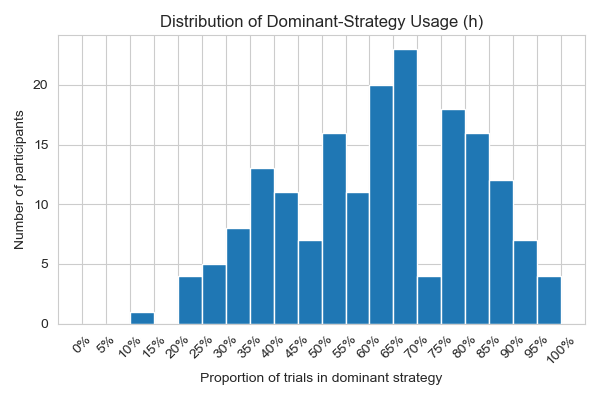
\includegraphics[width=\linewidth]{plots/strategies/dominant_prop_first_visits_area_screen_loc_h.png}}
          \end{subcaptionbox}
          \hfill
          \begin{subcaptionbox}{Proportion of trials most common strategy is used - Gatherers\label{fig:h2}}[0.45\textwidth]
            {\centering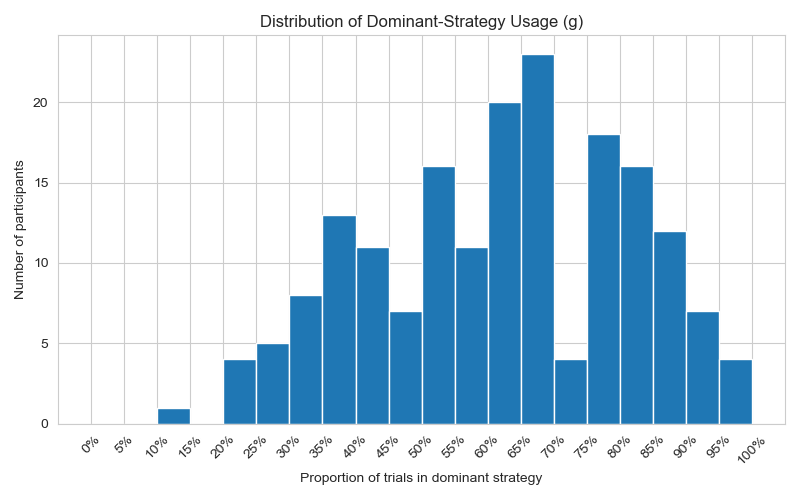
\includegraphics[width=\linewidth]{plots/strategies/dominant_prop_first_visits_area_screen_loc_g.png}}
          \end{subcaptionbox}
     \caption{Dominant Strategy Prevalence}
     \label{fig:dom_props}
    \end{figure}



    
    \subsection{Last Fixation}

    In a similar fashion to the First-Scan, we look at the order in which the segments are visited last, in hopes of finding a similar pattern to how the exploration ends. In Figure~\ref{fig:last_hunt_loc} we can see a similar pattern emerging to the one we see in First-Scan, with a clockwise scan-path. However, as indicated in Figure~\ref{fig:length} the common length of the Simplified Fixations Sequence is causing spillover. 

    \begin{figure}[H]
      \centering
      \begin{subcaptionbox}{Screen Location - A \label{fig:aaa}}[0.45\textwidth]
        {\centering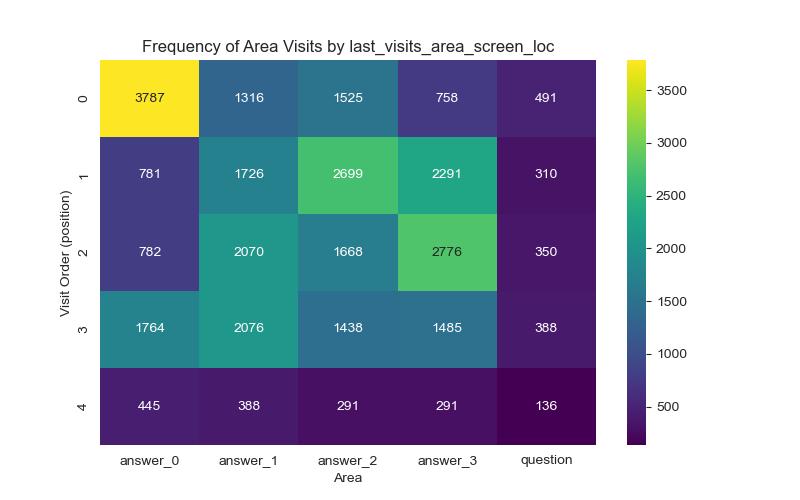
\includegraphics[width=\linewidth]{plots/visits/matrix__last_visits_area_screen_loc_hunters_A.png}}
      \end{subcaptionbox}
      \hfill
      \begin{subcaptionbox}{Screen Location - B\label{fig:bbb}}[0.45\textwidth]
        {\centering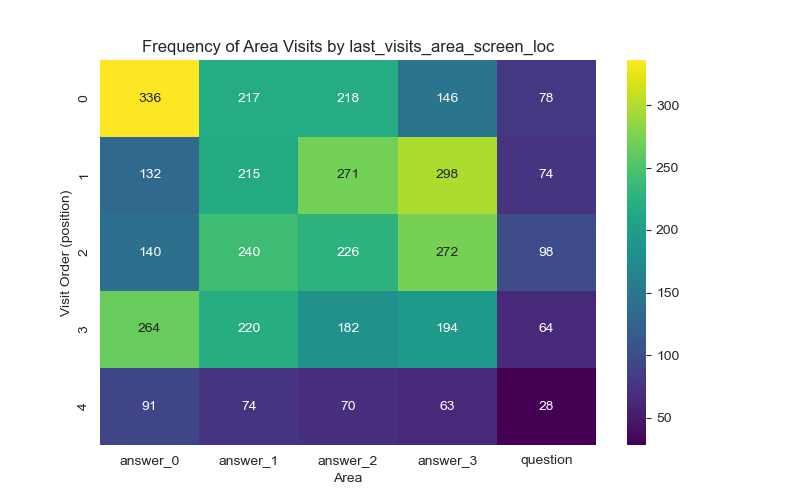
\includegraphics[width=\linewidth]{plots/visits/matrix__last_visits_area_screen_loc_hunters_B.png}}
      \end{subcaptionbox}
      
      \vspace{0.5em}
    
      \begin{subcaptionbox}{Screen Location - C\label{fig:ccc}}[0.45\textwidth]
        {\centering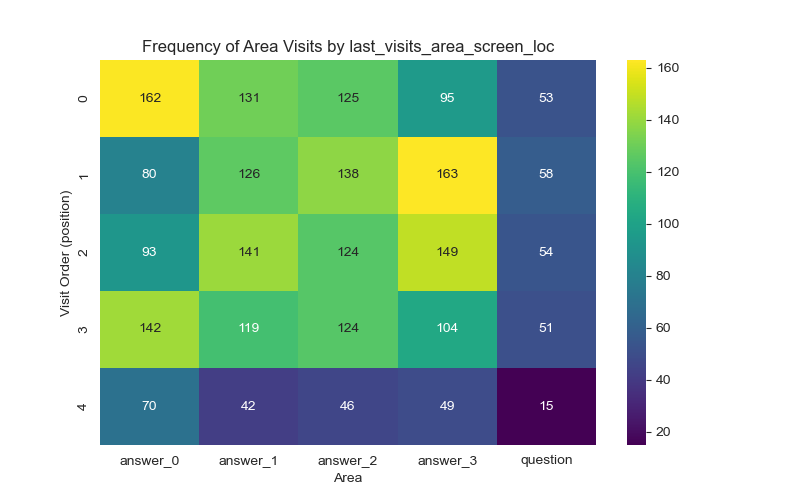
\includegraphics[width=\linewidth]{plots/visits/matrix__last_visits_area_screen_loc_hunters_C.png}}
      \end{subcaptionbox}
      \hfill
      \begin{subcaptionbox}{Screen Location - D\label{fig:ddd}}[0.45\textwidth]
        {\centering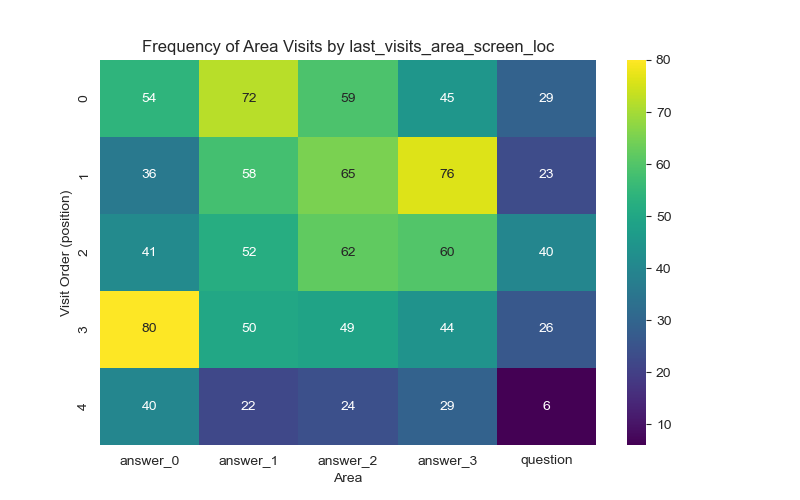
\includegraphics[width=\linewidth]{plots/visits/matrix__last_visits_area_screen_loc_hunters_D.png}}
      \end{subcaptionbox}
      
      \caption{Last Visits by Hunting Regime Participants}
      \label{fig:last_hunt_loc}
    \end{figure}

    \begin{figure}[H]
        \centering
        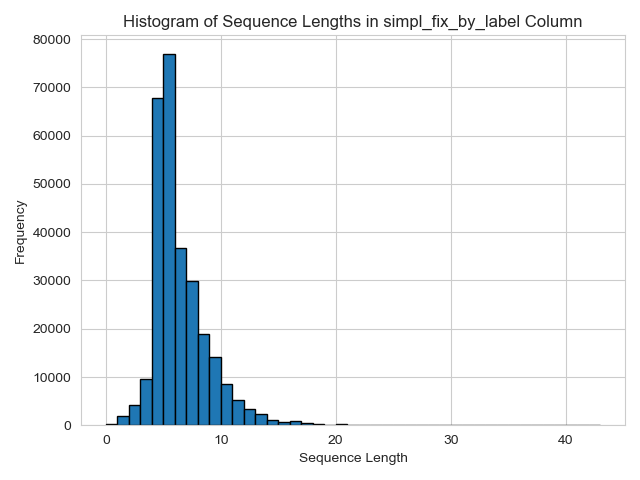
\includegraphics[width=0.75\linewidth]{plots/sequence_freq/simpl_fix_by_label.png}
        \caption{Simple Sequence Length}
        \label{fig:length}
    \end{figure}

    However, when looked at from the answer correctness perspective (Figure~\ref{fig:last_hunt_lbl}) we see clear indication of the last segment looked at being the answer selected. We find that 71.25\% of Gatherers and 68.24\% of Hunters have last area they visit be the answer they select.

    \begin{figure}[H]
          \centering
          % First row of images
          \begin{subcaptionbox}{Area Label - A \label{fig:a4}}[0.45\textwidth]
            {\centering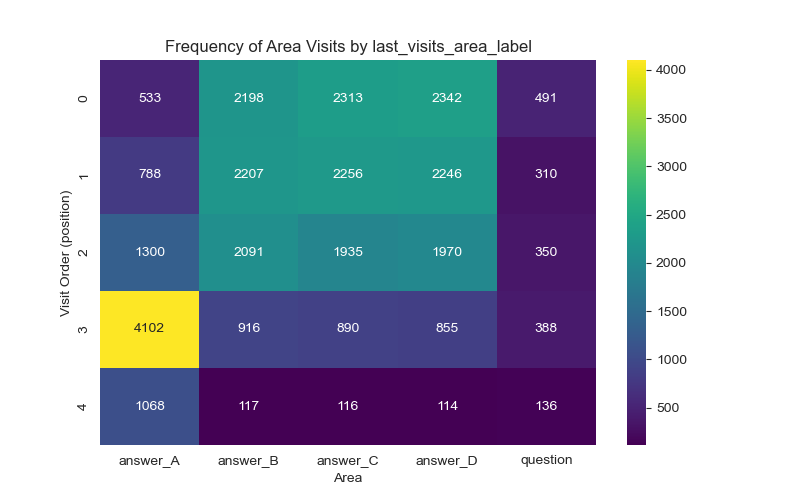
\includegraphics[width=\linewidth]{plots/visits/matrix__last_visits_area_label_hunters_A.png}}
          \end{subcaptionbox}
          \hfill
          \begin{subcaptionbox}{Area Label - B\label{fig:b4}}[0.45\textwidth]
            {\centering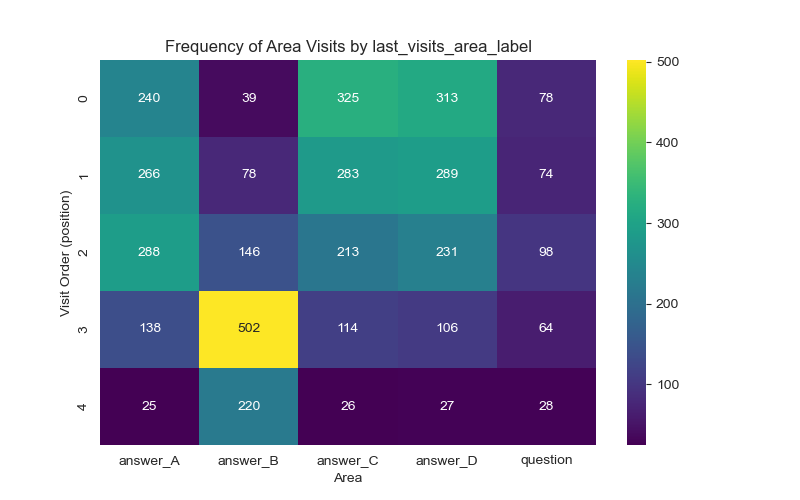
\includegraphics[width=\linewidth]{plots/visits/matrix__last_visits_area_label_hunters_B.png}}
          \end{subcaptionbox}
          
          \vspace{1em} % Vertical spacing between rows
        
          % Second row of images
          \begin{subcaptionbox}{Area Label - C\label{fig:c4}}[0.45\textwidth]
            {\centering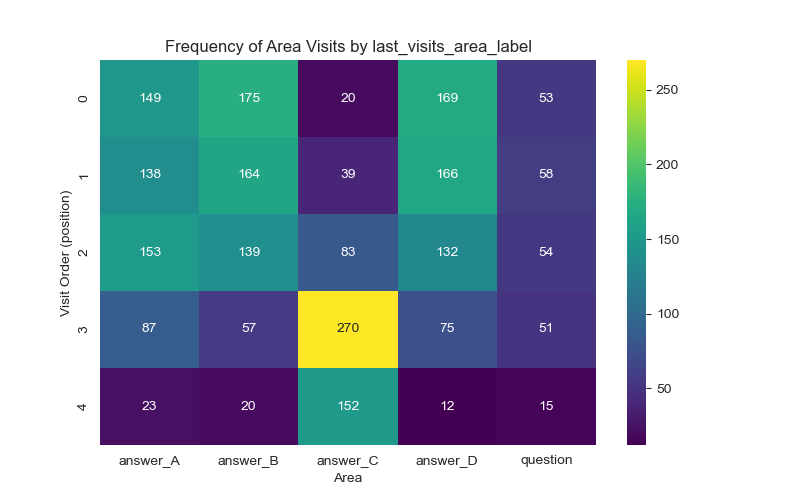
\includegraphics[width=\linewidth]{plots/visits/matrix__last_visits_area_label_hunters_C.png}}
          \end{subcaptionbox}
          \hfill
          \begin{subcaptionbox}{Area Label - D\label{fig:d4}}[0.45\textwidth]
            {\centering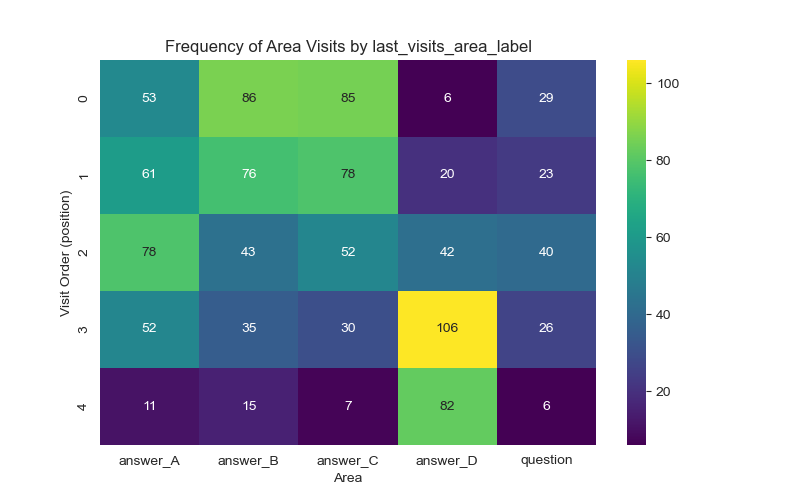
\includegraphics[width=\linewidth]{plots/visits/matrix__last_visits_area_label_hunters_D.png}}
          \end{subcaptionbox}
          
          \caption{Last Visits}
          \label{fig:last_hunt_lbl}
        \end{figure}
    
    
    \subsection{Mean Dwell Time by Selected Answer}

    We next examine whether participants spend disproportionately more time dwelling on the answer they ultimately choose, regardless of its screen location or correctness. For each experimental trial, we aggregate the IA dwell time for each of the five segments. We aim to access the dependency, or lack there of, between the attention given to the area and its Location or Label assignment, hoping to capture some inherent pattern in how participants distribute their attention between segments. 
 
    As indicated in Figure~\ref{fig:hun_dwell} (Hunters) and Figure~\ref{fig:gath_dwell} (Gatherers), both Hunting and Gathering regime participants showcase clear preference for an answer they end up selecting, with no dependence on the answers location or its objective correctness. This conclusion aligns with the research by Linder et. al. claiming gaze bias towards subjectively preferred answer options in multiple choice decision making \parencite{lindner2014tracking} as well as Tsai et. al. research claiming students pay more attention to chosen options rather then rejected ones \parencite{tsai2012visual}. We conclude no significant difference between Hunting and Gathering regimes.

        
        \begin{figure}[H]
          \centering
          \begin{subcaptionbox}{Answered A\label{fig:a5}}[0.45\textwidth]
            {\centering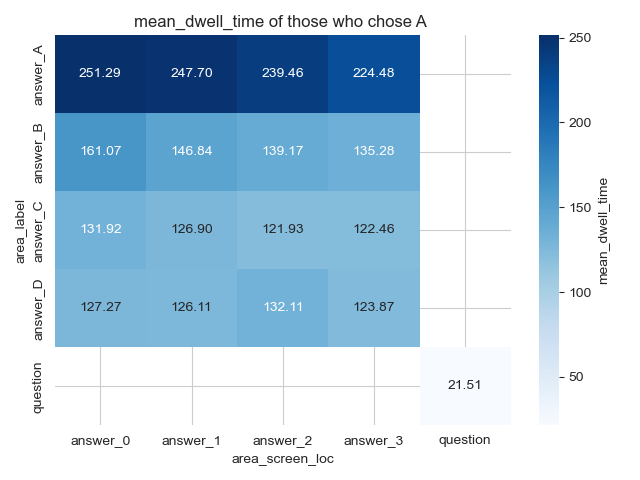
\includegraphics[width=\linewidth]{plots/matrix_plots/matrix_mean_dwell_time_A_hunters.png}}
          \end{subcaptionbox}
          \hfill
          \begin{subcaptionbox}{Answered B\label{fig:b5}}[0.45\textwidth]
            {\centering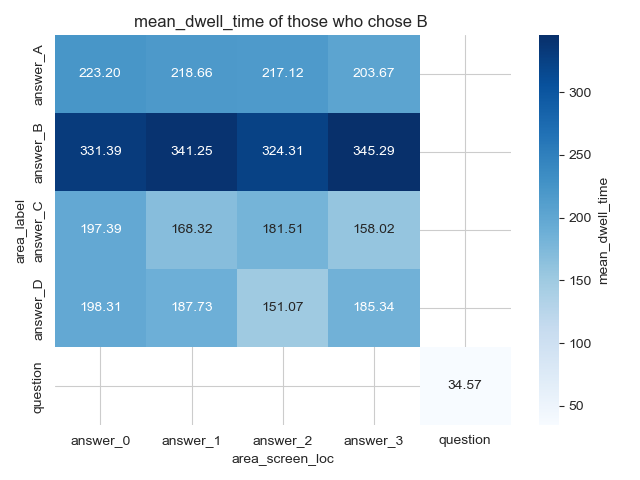
\includegraphics[width=\linewidth]{plots/matrix_plots/matrix_mean_dwell_time_B_hunters.png}}
          \end{subcaptionbox}
          
          \vspace{1em} 
        
          \begin{subcaptionbox}{Answered C\label{fig:C5}}[0.45\textwidth]
            {\centering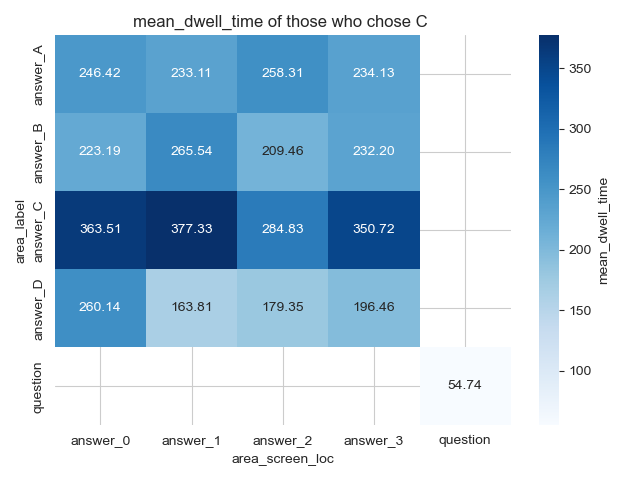
\includegraphics[width=\linewidth]{plots/matrix_plots/matrix_mean_dwell_time_C_hunters.png}}
          \end{subcaptionbox}
          \hfill
          \begin{subcaptionbox}{Answered D\label{fig:D5}}[0.45\textwidth]
            {\centering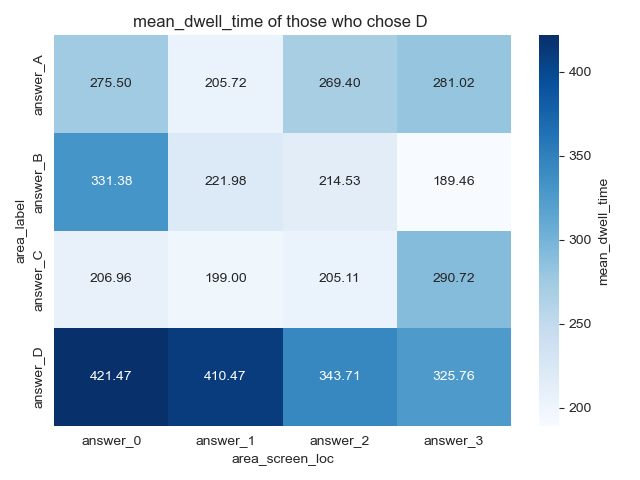
\includegraphics[width=\linewidth]{plots/matrix_plots/matrix_mean_dwell_time_D_hunters.png}}
          \end{subcaptionbox}
          
          \caption{HUNTERS - mean dwell time as dependent on area label (rows) and screen location (columns) separated by the selected answer in a given trial (by correctness)}
          \label{fig:hun_dwell}
        \end{figure}


        \begin{figure}[H]
          \centering
          \begin{subcaptionbox}{Answered A\label{fig:A6}}[0.45\textwidth]
            {\centering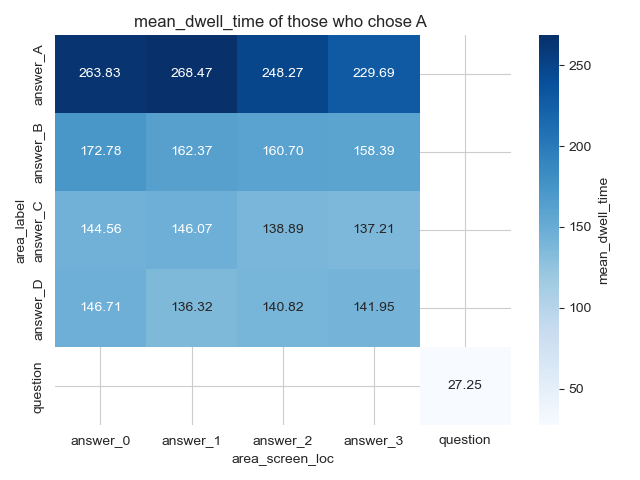
\includegraphics[width=\linewidth]{plots/matrix_plots/matrix_mean_dwell_time_A_gatherers.png}}
          \end{subcaptionbox}
          \hfill
          \begin{subcaptionbox}{Answered B\label{fig:B6}}[0.45\textwidth]
            {\centering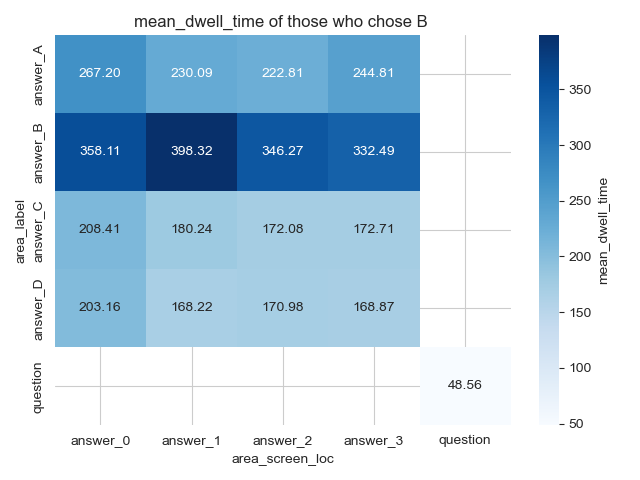
\includegraphics[width=\linewidth]{plots/matrix_plots/matrix_mean_dwell_time_B_gatherers.png}}
          \end{subcaptionbox}
          
          \vspace{1em} 
        
          \begin{subcaptionbox}{Answered C\label{fig:C6}}[0.45\textwidth]
            {\centering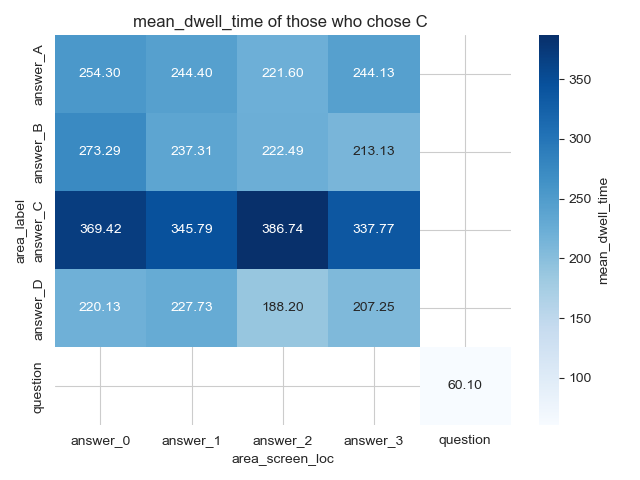
\includegraphics[width=\linewidth]{plots/matrix_plots/matrix_mean_dwell_time_C_gatherers.png}}
          \end{subcaptionbox}
          \hfill
          \begin{subcaptionbox}{Answered D\label{fig:D6}}[0.45\textwidth]
            {\centering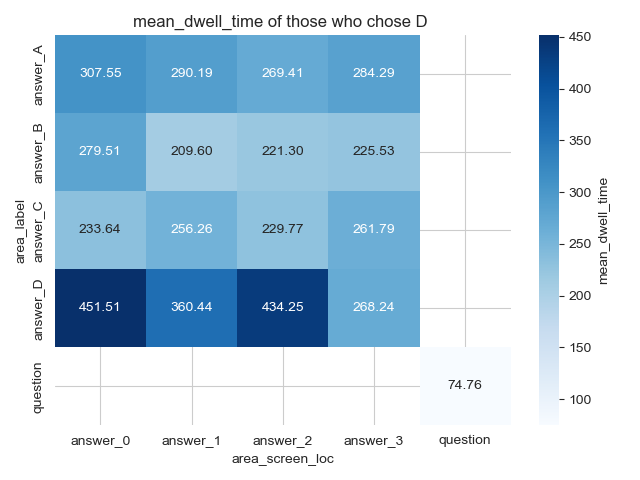
\includegraphics[width=\linewidth]{plots/matrix_plots/matrix_mean_dwell_time_D_gatherers.png}}
          \end{subcaptionbox}
          
          \caption{GATHERERS - mean dwell time as dependent on area label (rows) and screen location (columns) separated by the selected answer in a given trial (by correctness)}
          \label{fig:gath_dwell}
        \end{figure}




\section{Discussion}
Our analysis of eye‐tracking data from the OneStop multiple‐choice experiment reveals several convergent findings. First, participants in both the Hunting and Gathering regimes overwhelmingly adopt a clockwise scanning heuristic, beginning at the topmost option and proceeding around the diamond‐shaped layout. Second, individual participants tend to repeat one dominant first‐scan strategy across trials rather than randomly varying their scanning order. Third, the final fixation within each trial most frequently falls on the answer that participants ultimately select—approximately 68\% of Hunters and 71\% of Gatherers end their scan on their chosen option. Finally, mean dwell‐time analyses confirm a robust gaze bias: participants spend significantly more time fixating on the region corresponding to their final answer, regardless of whether they knew the question in advance (Hunters) or encountered it only after reading the passage (Gatherers).

\subsection*{First‐Scan Heuristics and Consistent Strategies}
Our research demonstrates the prevalence of a clockwise first-scan pattern. Participants appear to impose a simple spatial heuristic (clockwise from the top) whenever they face a diamond‐shaped option layout. This finding suggests that, when no immediate semantic cues to differentiate the four choices, individuals rely on a spatial strategy that reduces cognitive load.

Moreover, our measure of each participant’s “dominant strategy”—the four‐element scan sequence most frequently used across trials—shows that over 58\% of Hunters and over 72\% of Gatherers adhered to the same first‐scan order in at least half of their trials. In other words, once a participant selects a preferred scanning path, they tend to repeat it rather than explore alternative orders. 

\subsection*{Last Fixation and Gaze Bias}
Participants’ final fixation overwhelmingly falls on the answer they ultimately choose. Specifically, in 68.2\% of Hunting trials and 71.3\% of Gathering trials, the last IA visited corresponds to the chosen response. The strong link between final fixation and eventual response suggests that eye‐tracking can serve as a real‐time proxy for emerging preferences in multiple‐choice tasks.


\subsection*{Dwell Time Across Answer Regions}
Beyond the final fixation, our aggregated dwell‐time matrices (Figure~\ref{fig:gath_dwell} and Figure~\ref{fig:hun_dwell}) show a clear preference: regardless of regime or answer correctness, participants devote longer total fixation time to the option they will ultimately choose. In both Hunters and Gatherers, the mean dwell time on the chosen segment is on average higher than on the most‐visited distractor. This dwell‐time preference is consistent with earlier studies \parencite{lindner2014tracking} \parencite{tsai2012visual}.


\section{Limitations}
Despite the insights we find, our study has several limitations:

Simplified Sequences Ignore Within‐Segment Fixation Patterns: By collapsing consecutive fixations in the same segment into a single visit, we focus exclusively on scanning order rather than fixation duration. Additionally, our concentration of first-visits order ignores dynamics (e.g., revisits to the same option). While this simplification facilitates cross-trial comparisons in a consistent way, and reduces scan-sequence noise, it discards potentially informative patterns.

Diamond Layout Specificity: Our findings derive from a four-option interface arranged in a diamond shape controlled by a D-pad. It is possible that a grid layout, linear list, or randomized button-mapping would lead to different scan heuristics. 


\section{Conclusions}
In sum, our results demonstrate that—in a four-option, diamond-shaped multiple-choice environment—participants adopt a simple clockwise first-scan heuristic, repeatedly apply that strategy within sessions, and exhibit strong final-fixation and dwell-time biases toward the chosen response. These patterns hold regardless of whether participants see the question before or after reading the passage, suggesting that gaze bias and scan consistency are robust features of multiple-choice decision making. By combining scan‐order analysis with dwell‐time metrics, our study adds new evidence that eye‐tracking can illuminate the subtle dynamics of choice behavior and offers practical validity checks for assessment design.

\printbibliography


\newpage
\appendix
\begin{appendices}
    \section{Fixation‐Sequence Visualization}
    \label{app:fixseq}
    
    \begin{figure}[H]
      \centering
      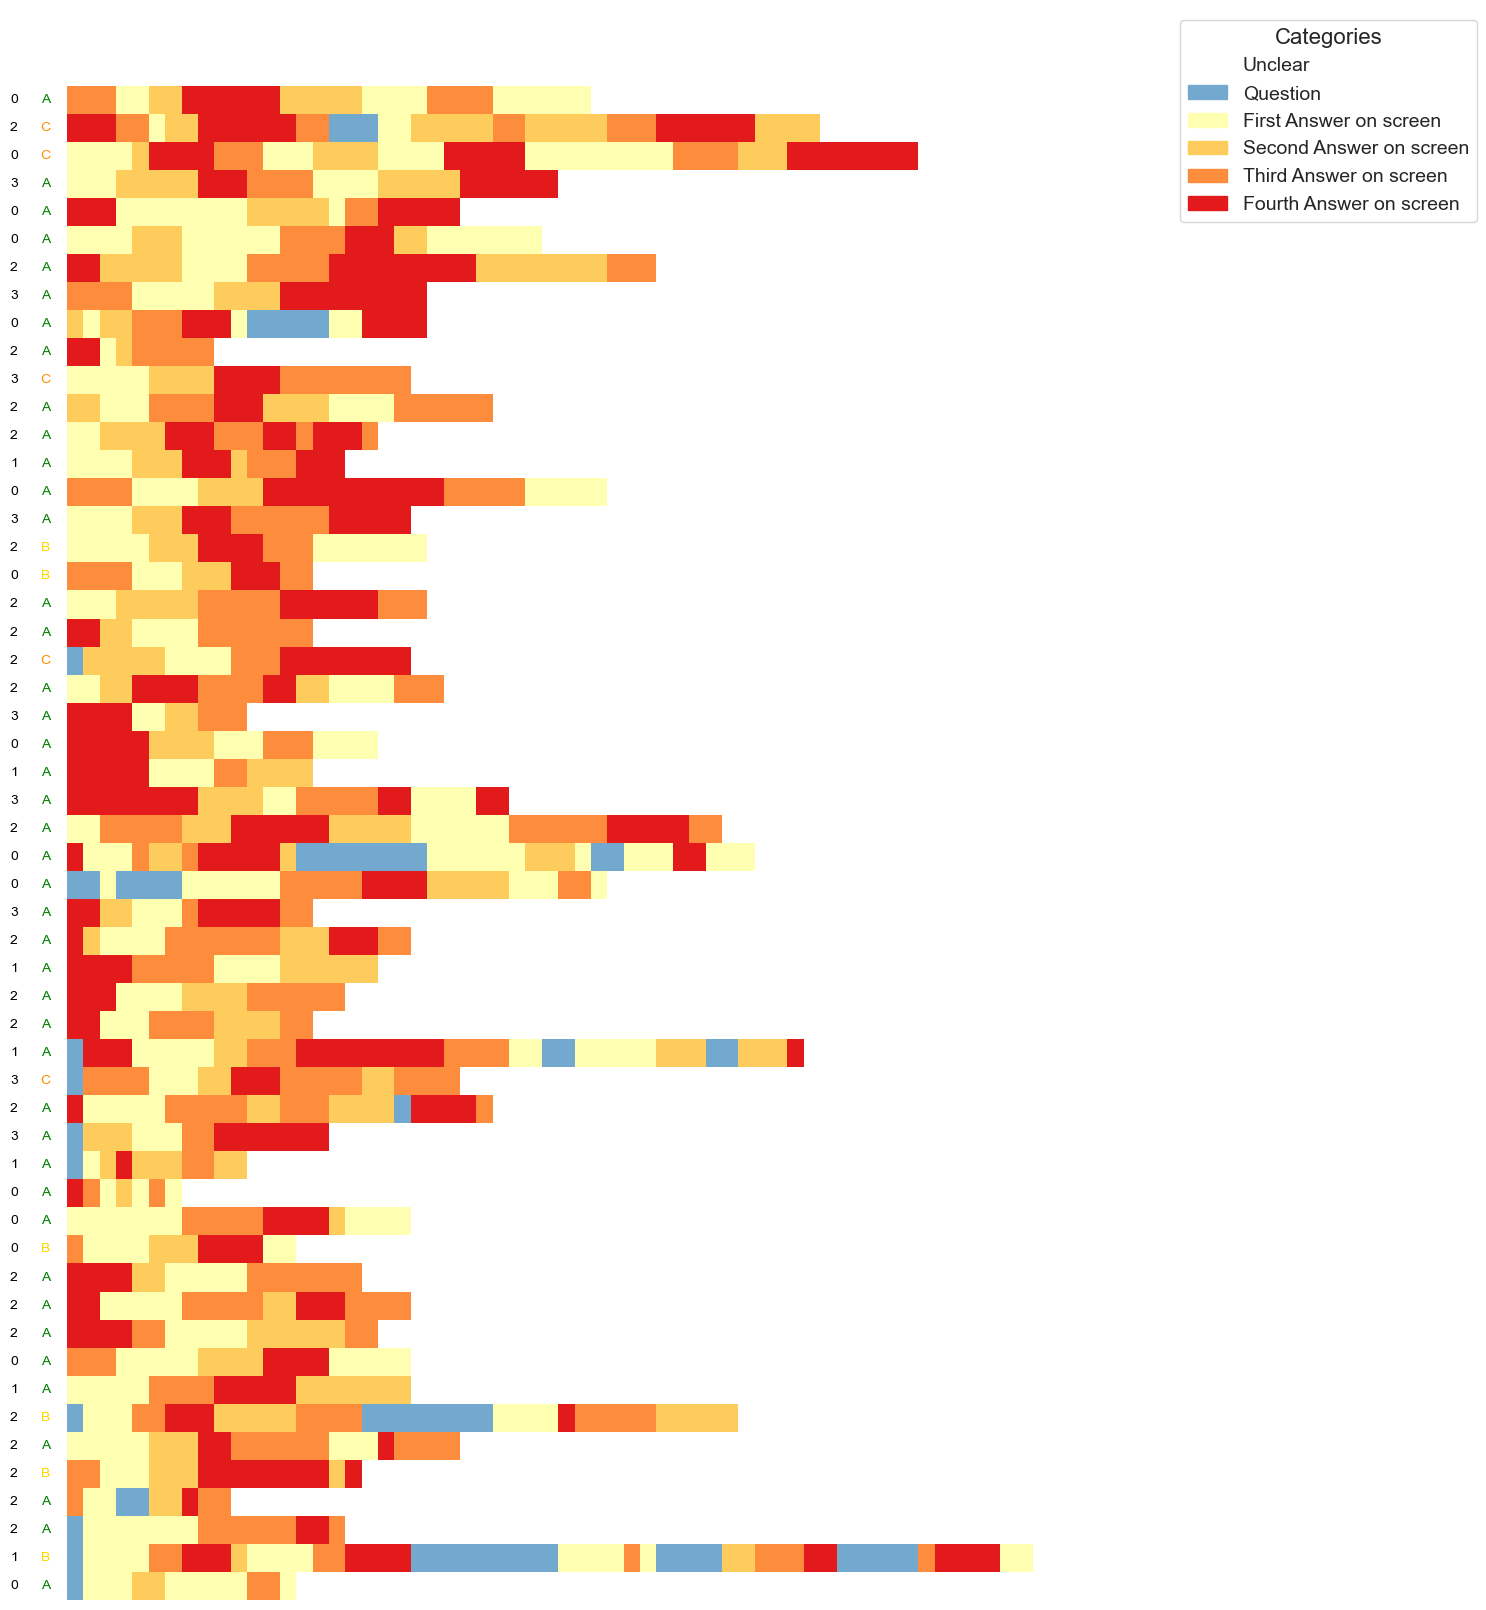
\includegraphics[width=1\textwidth]{plots/random_p_by_loc.png}
      \caption{Example fixation sequence for one participant (by screen location). Each fixation is a single colored rectangle. First column (numbers) indicates the location of the correct answer. Second column (letters) indicates the answer selected in this trial.}
      \label{fig:fixseq1}
    \end{figure}
    
    \begin{figure}[H]
      \centering
      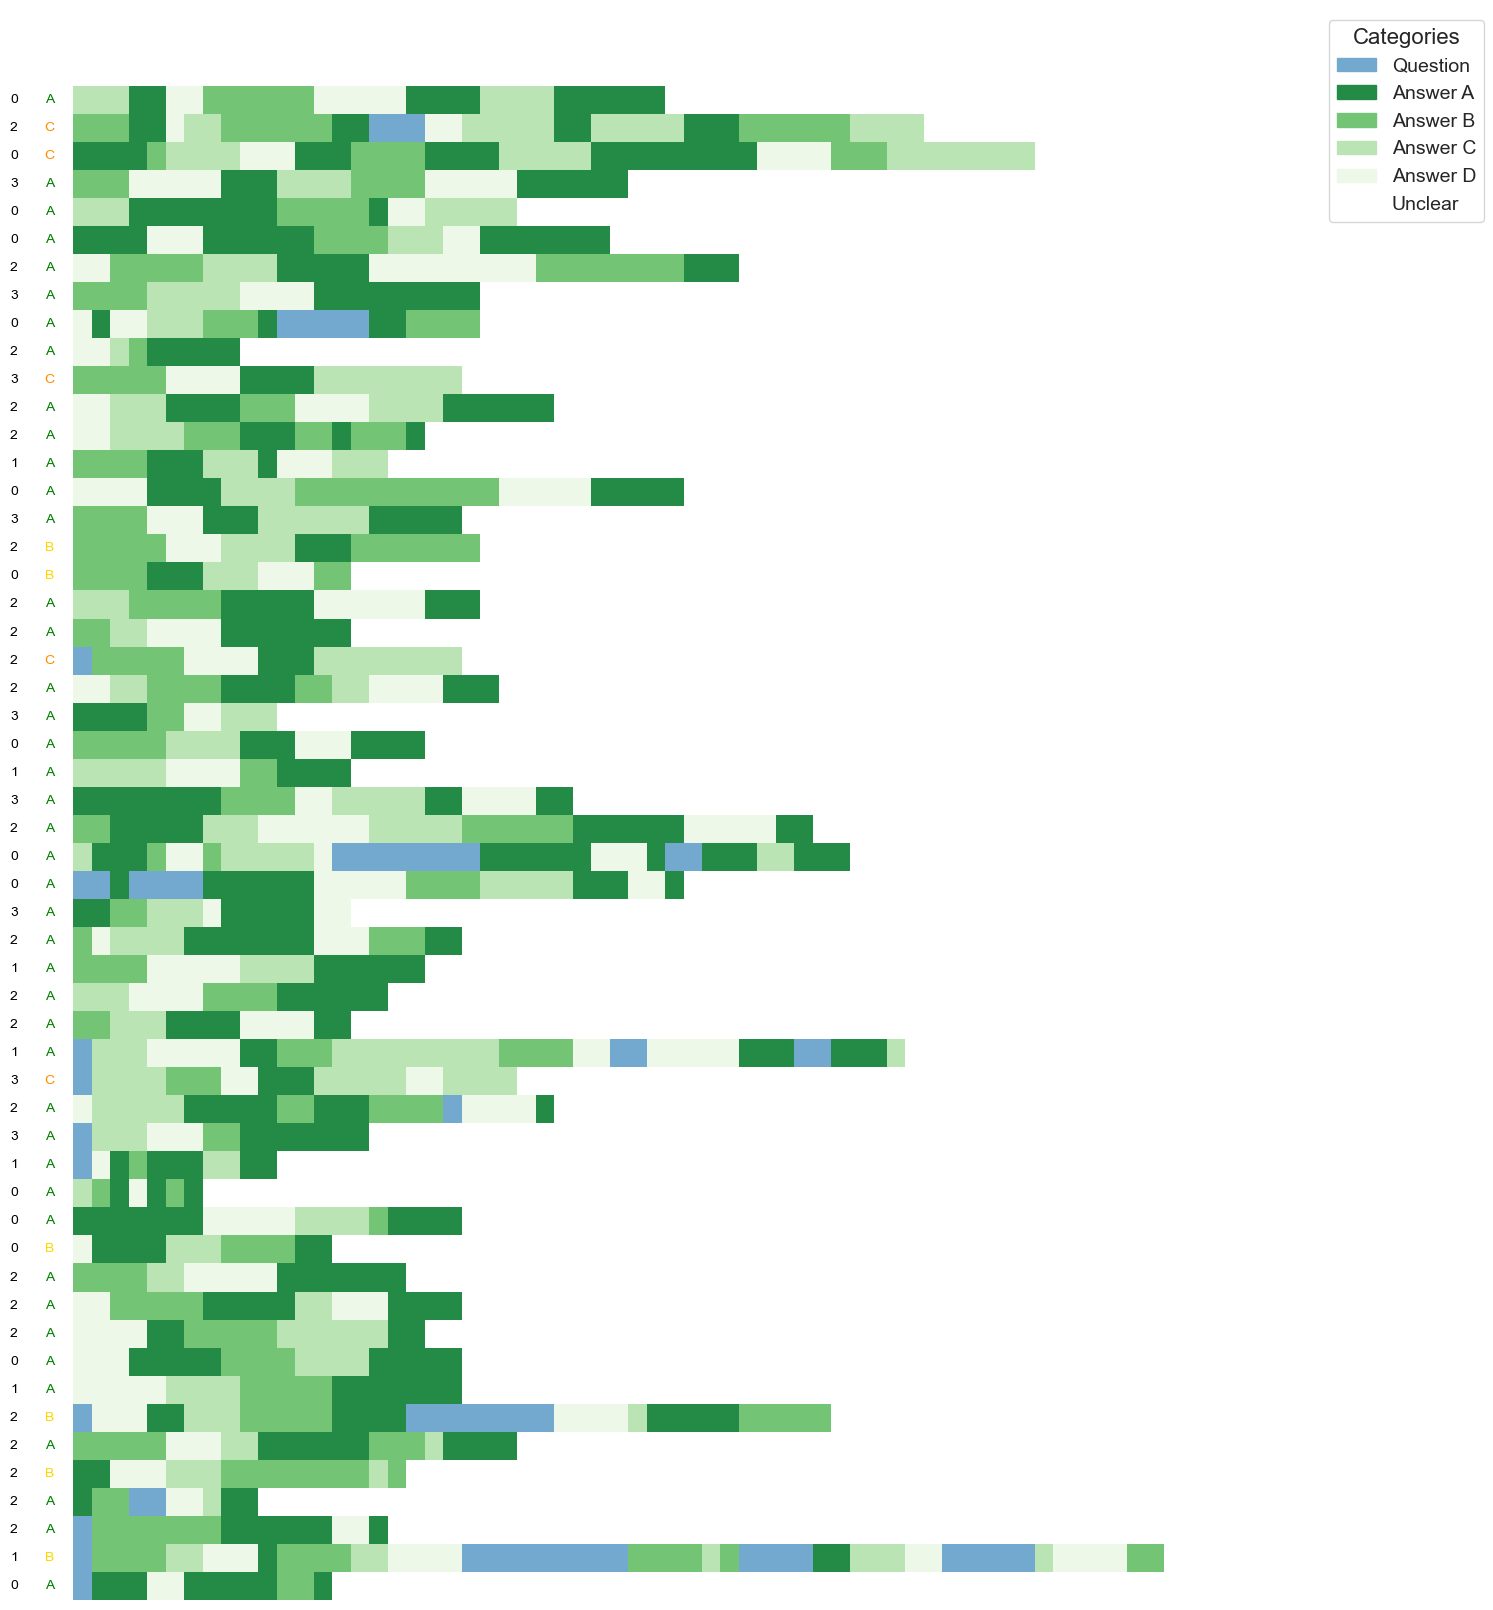
\includegraphics[width=1\textwidth]{plots/random_p_by_lbl.png}
      \caption{Example fixation sequence for one participant (by area label). Each fixation is a single colored rectangle. First column (numbers) indicates the location of the correct answer. Second column (letters) indicates the answer selected in this trial.}
      \label{fig:fixseq2}
    \end{figure}


    \section{Location-based lag-1 Z-score matrix}
    \label{app:lsa_location}
    \begin{table}[H]
        \centering
        \begin{tabular}{lrrrr}
        \hline
                    & \textbf{answer\_0}  & \textbf{answer\_1}   & \textbf{answer\_2}   & \textbf{answer\_3}   \\ 
        \hline
        \textbf{answer\_0}  &   --        &   154.645   &   436.987   &  -323.095   \\
        \textbf{answer\_1}  &  285.501    &    --       &  -116.050   &   241.728   \\
        \textbf{answer\_2}  &  101.319    &  -204.647   &    --       &   549.927   \\
        \textbf{answer\_3}  &  -32.138    &   392.883   &    87.278   &    --       \\
        \hline
        \end{tabular}
        \caption{Lag-1 standardized residuals (“Z”‐scores) for screen‐location transitions. Each cell $(i,j)$ shows $Z_{ij}$ for the transition from \textit{answer\_i} to \textit{answer\_j}. Diagonal entries are omitted (structural zeros).}
        \label{tab:lsa_location}
    \end{table}


    \section{Correctness-based lag-1 Z-score matrix}
    \label{app:lsa_label}
    \begin{table}[H]
        \centering
        \begin{tabular}{lrrrr}
        \hline
                    & \textbf{answer\_A}   & \textbf{answer\_B}   & \textbf{answer\_C}   & \textbf{answer\_D}   \\ 
        \hline
        \textbf{answer\_A}  &   --       &   204.143   &   164.875   &   159.109   \\
        \textbf{answer\_B}  &  189.746   &    --       &   102.256   &    80.206   \\
        \textbf{answer\_C}  &  145.300   &    85.453   &    --       &   116.036   \\
        \textbf{answer\_D}  &  138.391   &   101.411   &    95.553   &    --       \\
        \hline
        \end{tabular}
        \caption{Lag-1 standardized residuals (“Z”‐scores) for correctness‐based transitions. Each cell $(i,j)$ shows $Z_{ij}$ for the transition from \textit{answer\_i} to \textit{answer\_j}. Diagonal entries are omitted (structural zeros).}
        \label{tab:lsa_label}
    \end{table}
    
\end{appendices}

\end{document}

